\section{Evaluation}

%%%%%%%%%%%%%%%%%%%%%%%%%%%%%%%%%%%%%%%%%%%%%%%%%%%%%%%%%%%%%%%%%%%%%%%%%%%%%%%%
\subsection{nix}
%%%%%%%%%%%%%%%%%%%%%%%%%%%%%%%%%%%%%%%%%%%%%%%%%%%%%%%%%%%%%%%%%%%%%%%%%%%%%%%%
\begin{frame}
  \frametitle{Evaluation}
\begin{itemize}

	\item We wanted to rigorously compare our results with the results from the original paper.
	\item But: no implicit datasets available!

	\item We had to implement a special random number generator (RNG) and a benchmark generator from pseudocode delivered by \cite[Taillard'03]{Benchmarks}.

	\item The benchmarks were reproduced based on given seeds for the RNG.
\end{itemize}

\end{frame}

%%%%%%%%%%%%%%%%%%%%%%%%%%%%%%%%%%%%%%%%%%%%%%%%%%%%%%%%%%%%%%%%%%%%%%%%%%%%%%%%

\begin{frame}
	\frametitle{Evaluation method}
\begin{itemize}

	\item We considered benchmark problems of sizes
		\begin{itemize}
		
			\item 4x4 (4 jobs, 4 machines), 5x5, 7x7, 10x10, 15x15, 20x20. 
		\end{itemize}
		
	For each problem, we  ran all 3 algorithms for \textbf{200} generations with a population size of \textbf{200}.

	\item 	Since different runs produce different results, we repeated each run \textbf{100} times. 
	\\ 		\textcolor{red}{\textrightarrow		High computational cost!}

	\item 	Complexity increases with rising problem size \textrightarrow	only a few large problems evaluated 
\end{itemize}

	
\end{frame}

%%%%%%%%%%%%%%%%%%%%%%%%%%%%%%%%%%%%%%%%%%%%%%%%%%%%%%%%%%%%%%%%%%%%%%%%%%%%%%%%
%\subsection{Results}
%%%%%%%%%%%%%%%%%%%%%%%%%%%%%%%%%%%%%%%%%%%%%%%%%%%%%%%%%%%%%%%%%%%%%%%%%%%%%%%%

\begin{frame}
  \frametitle{Results}
	\vspace{-1.8cm}
\begin{figure}[htbp]
	\centering
	\hspace{1cm}
		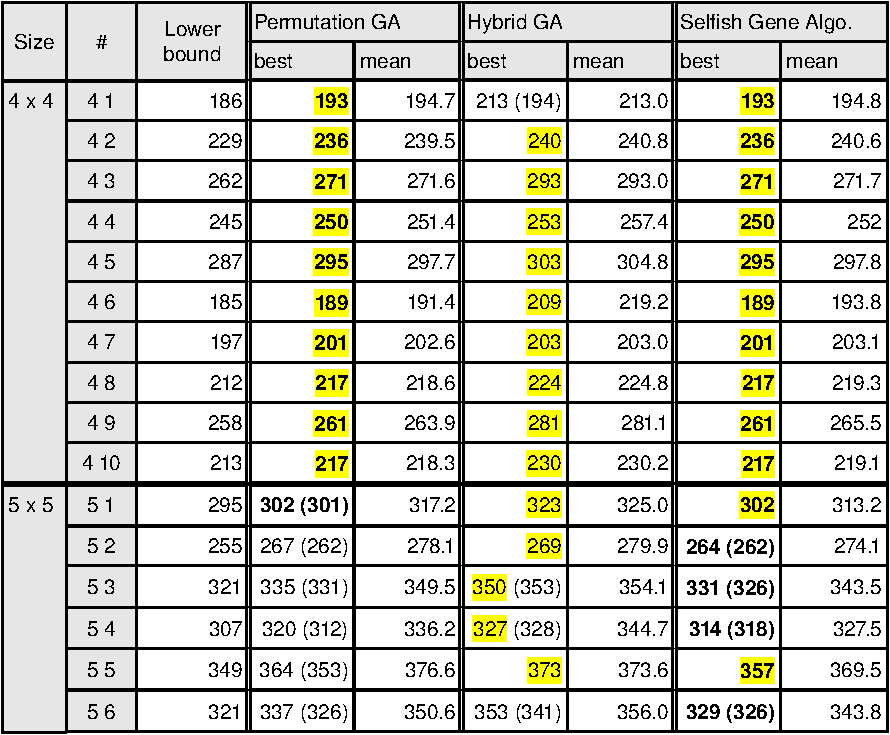
\includegraphics[scale=.5]{images/results1.pdf}
	\caption{We reached the best known solution for all 4x4 problems. For medium problems (5x5, 7x7), the Selfish Gene Algorithm performs best.}
	\label{fig:label}
\end{figure}
\end{frame}

%%%%%%%%%%%%%%%%%%%%%%%%%%%%%%%%%%%%%%%%%%%%%%%%%%%%%%%%%%%%%%%%%%%%%%%%%%%%%%%%

\begin{frame}
  \frametitle{Results (2)}

\begin{figure}[htbp]
	\centering
		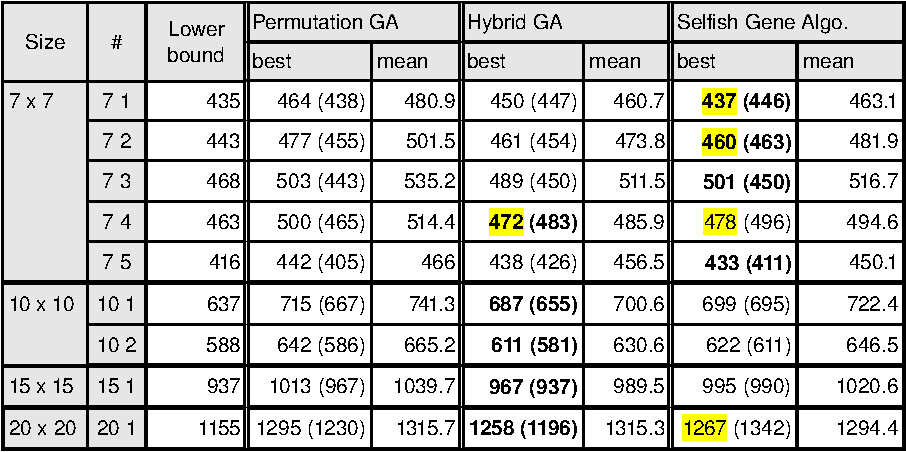
\includegraphics[scale=.5]{images/results2.pdf}
	\caption{The gap between lower bounds and found solutions increases with the problem size. For large problems, the hybrid GA performs best.}
	\label{fig:label}
\end{figure}
\end{frame}

%%%%%%%%%%%%%%%%%%%%%%%%%%%%%%%%%%%%%%%%%%%%%%%%%%%%%%%%%%%%%%%%%%%%%%%%%%%%%%%%

\begin{frame}
	\frametitle{Results (3)}
\begin{itemize}

	\item 	We matched the best known results for small problems.

	\item 	We found acceptable solutions for larger problems, but
		\begin{itemize}
			\item 		we implemented our own library instead of using a well known optimization library
			\item 		therefore implementations of functions like \emph{crossover} may differ
		\end{itemize}
		

	\item 	Neither our nor the original implementation matched the results of \cite[PSO'08]{PSO}.
\end{itemize}

	
\end{frame}

%%%%%%%%%%%%%%%%%%%%%%%%%%%%%%%%%%%%%%%%%%%%%%%%%%%%%%%%%%%%%%%%%%%%%%%%%%%%%%%%

\begin{frame}
  \frametitle{Convergence}
\end{frame}

%%%%%%%%%%%%%%%%%%%%%%%%%%%%%%%%%%%%%%%%%%%%%%%%%%%%%%%%%%%%%%%%%%%%%%%%%%%%%%%%
